% Chapter 55: Light and Atoms Working Together
\chapter{Light and Atoms Working Together}

\step{A Counterintuitive Opening}

\begin{mainline}
% BEGIN TRANSLATOR SAFETY NOTE
\textbf{Translator safety note:} Do not aim lasers outdoors or toward people, animals, vehicles, or aircraft. Prefer a recorded comparison; any instructor-run indoor demonstration needs a controlled beam ending on a matte surface, away from eyes and reflections. See \href{https://www.fda.gov/consumers/consumer-updates/laser-toys-how-keep-kids-safe}{FDA laser safety guidance}.
% END TRANSLATOR SAFETY NOTE

Take an ordinary inexpensive red laser pointer and a flashlight, using similar batteries and milliwatt-to-watt powers. At night aim both at a wall twenty meters away. The flashlight spreads a fuzzy one- or two-meter pancake, while the laser makes a dazzling fingernail-sized spot. Compare colors with an old disc: flashlight white unfolds into a full rainbow; laser red is almost impurity-free. Like a choir singing one note in perfect time versus a thousand market voices, they contrast order and disorder. Unlike human singers who still drift after rehearsals, lasers obtain order from a physical law.

Your bedroom may hold a second phenomenon: glow-in-the-dark ceiling stars. After illumination they glow faintly for ten or more minutes in darkness, storing light like coins to spend slowly. Stranger, dazzling red hardly feeds them, while much dimmer violet fills them immediately. Bright loses to dim.

Both reflect selective, organizable atomic light exchange. Familiar appearances include banknote security fluorescence, white shirts glowing blue under dance-floor violet lamps, sodium canopy lights, traffic lights, and white phone-flash LEDs. Every artificial source follows atomic absorption and emission rules. We will trace their cooperation through fluorescence, lasers, spectroscopy, and atomic clocks.
\end{mainline}

\step{Make a Guess First}

\begin{mainline}
Stake your intuitions before reading answers:

\begin{itemize}[leftmargin=1.8em]
  \item Is laser purity due to sophisticated filters, an inherently single-color material, or something else?
  \item Is its narrow beam due to especially orderly emitting points?
  \item Does a glowing sticker resemble a slowly reflecting mirror or a rechargeable battery?
  \item Does red versus violet charging depend on total light or each photon's denomination?
\end{itemize}

Write answers for later comparison. Physicists often lose such bets too: early-twentieth-century experts collectively expected more detailed electromagnetism to balance atomic accounts. The ancestors of your laser pointer forced them to rewrite those accounts instead.
\end{mainline}

\step{Hands-on Experiment}

\begin{experiment}[Disc Spectra and Fluorescent Water]
Prepare an old CD or DVD, red laser pointer, yellow highlighter, transparent cup, and glowing sticker; a banknote-checking violet lamp or violet LED helps. Safety: never point lasers at eyes, and beware mirror and tile reflections.

% BEGIN TRANSLATOR SAFETY NOTE
\textbf{Translator safety note:} Use recorded demonstrations for the laser-through-glass steps: the cup, liquid surface, and disc can redirect beams unexpectedly. Do not increase laser power to obtain the stated color change. Prefer a visible LED for sticker comparisons, never a UV germicidal lamp; avoid direct eye or skin exposure to UV. See \href{https://www.fda.gov/consumers/consumer-updates/laser-toys-how-keep-kids-safe}{FDA laser guidance} and \href{https://www.fda.gov/radiation-emitting-products/tanning/ultraviolet-uv-radiation}{FDA UV guidance}.
% END TRANSLATOR SAFETY NOTE

Step one: build a crude spectroscope. Dim the room and illuminate the disc with an incandescent or halogen lamp, rotating it to find the reflected rainbow. Repeat with an LED desk lamp or compact fluorescent. Incandescent light is continuous; LEDs and compact fluorescents show separated bright bands with black between. One disc reveals two distinct light identities.

Step two: change color in water. Soak and stir a yellow highlighter's ink core in half a cup, making pale yellow-green water. In darkness send the red laser horizontally through the side: a bright green path appears. Red enters, green leaves; the water changes color.

Step three: compare charging. Illuminate one half of a sticker closely with a red laser or LED for thirty seconds, the other with violet, a banknote lamp, violet LED, or window sunlight, for thirty seconds. Compare in darkness: violet's corner glows more; prolonged red hardly charges it.

Record whether spectra are continuous or discrete, whether fluorescence is bluer than incident light, and which light charges the sticker. These are our experimental foundations.
\end{experiment}

\step{The Old Model Runs into Trouble}

\begin{mainline}
Before Chapter 51, light was continuously divisible electromagnetic energy and atoms miniature orbiting-electron solar systems. Four accounts now fail.

First, the account itself is bankrupt. Chapter 51's orbiting electrons radiate, lose energy, and collapse into nuclei in far less than a second. Stable atoms cannot be miniature solar systems with such definite trajectories.

Second, continuous rainbows cannot explain discrete bands. Hot solid filaments emit continuously; dilute neon, mercury in compact fluorescents, and fireworks strontium and copper give fixed thin lines, unique elemental fingerprints. Scatter salt into a blue stove flame and brilliant sodium yellow appears, the same note as old sodium streetlights. Infinitely divisible continuous light cannot explain only a few notes.

% BEGIN TRANSLATOR SAFETY NOTE
\textbf{Translator safety note:} Do not reproduce the stove-flame invitation above. Use a recorded flame test or an instructor-run demonstration with suitable equipment and splash goggles; never add flammable solvents. See \href{https://institute.acs.org/acs-center/lab-safety/education-training/safer-experiments/flame-test.html}{ACS flame-test safety guidance}.
% END TRANSLATOR SAFETY NOTE

Third, fluorescence: red in, green out. An undifferentiated energy stream should not change color only one way. You never see stickers turn green into blue; nature does not reverse the direction.

Fourth, denomination discrimination: intense red cannot charge what dim violet can. If only total energy matters, this is absurd, unless atoms inspect each packet's value rather than the total. Wrong denominations cannot buy the ticket however much small change you bring.

Chapter 42's blackbody and photoelectric lessons leave one exit: discrete atomic energies exchange whole light packets, each denomination set by color. These are our new concepts.
\end{mainline}

\step{Inventing New Concepts}

\begin{mainline}
First, energy levels. Atomic energy is stairs, not a ramp: discrete rungs require whole jumps. Unlike real stairs permitting a pause between steps, atoms have no intermediate-level states even momentarily. Nor are levels planetary orbits: Chapter 52 assigns energy, not position or a definite route.

Second, absorption and spontaneous emission. A low-level atom can swallow a photon exactly matching a gap and rise. Neither too little nor too much is accepted: no small change, no change returned. An excited atom randomly jumps down at an unpredictable instant, emitting one gap-sized photon. Neon orange-red and fireworks strontium red or copper blue-green are fixed denominations. Individual timing is fundamentally unpredictable, Chapter 45's probability again, but immense ensembles are statistically stable enough for clocks, as we will discuss.

Third, stimulated emission. In 1916--1917 Einstein's radiation-equilibrium account required another process: a matching photon passing an excited atom can invite immediate descent and a second photon, alongside the possibility of lower-state absorption. Crucially, the new photon matches frequency, direction, and phase, a perfect clone. Like an avalanche, one snowball recruits more. Unlike mechanical snowball collisions, photons do not knock photons out of atoms; a conductor's synchronized downbeat is closer, with no off-key clone at all. Separate levels: lasers and discrete spectra are experimental facts; transitions plus photon cloning are the model's simplest unfailing account.
\end{mainline}

\begin{figure}[htbp]
\centering
\begin{tikzpicture}[>=Stealth,scale=0.95]
% ---- Absorption ----
\draw[thick] (0,0)--(1.8,0); \draw[thick] (0,1.5)--(1.8,1.5);
\fill (0.9,0) circle (1.6pt);
\draw[decorate,decoration={snake,amplitude=1.2pt,segment length=5pt},->] (-0.7,-0.6)--(0.75,1.2);
\node at (0.9,-1.0) {Absorption};
% ---- Spontaneous emission ----
\draw[thick] (3.4,0)--(5.2,0); \draw[thick] (3.4,1.5)--(5.2,1.5);
\fill (4.3,1.5) circle (1.6pt);
\draw[->,dashed] (4.3,1.35)--(4.3,0.15);
\draw[decorate,decoration={snake,amplitude=1.2pt,segment length=5pt},->] (4.5,0.75)--(6.0,-0.2);
\node at (4.3,-1.0) {\shortstack{Spontaneous\\emission}};
% ---- Stimulated emission ----
\draw[thick] (7.0,0)--(8.8,0); \draw[thick] (7.0,1.5)--(8.8,1.5);
\fill (7.9,1.5) circle (1.6pt);
\draw[decorate,decoration={snake,amplitude=1.2pt,segment length=5pt},->] (6.2,0.9)--(7.6,0.9);
\draw[decorate,decoration={snake,amplitude=1.2pt,segment length=5pt},->] (8.1,1.05)--(9.7,1.05);
\draw[decorate,decoration={snake,amplitude=1.2pt,segment length=5pt},->] (8.1,0.7)--(9.7,0.7);
\node at (7.9,-1.0) {\shortstack{Stimulated\\emission}};
\end{tikzpicture}
\caption{Three atomic light transactions. Dots mark occupied levels; wavy arrows are photons. In stimulated emission one arrives and two identical photons leave.}
\end{figure}

\begin{mainline}
Fourth, population inversion. The same invitation produces low-state absorption and high-state emission symmetrically. Thermal equilibrium usually has more downstairs, so absorption beats amplification. Gain requires more upstairs than downstairs, population inversion. Pumping supplies energy through current or another beam, like pumping water into a high reservoir. Energy is stored first then released, never created: every unit comes from the supply. A practical third-level route pumps rapidly into a short-lived high state, which quickly falls into a long-lived metastable waiting room, accumulating inversion relative to the lower level.

Fifth, fluorescence and phosphorescence. Absorbed ultraviolet lifts a molecule high; internal transfers convert some energy into vibration and heat before a lower transition emits visible light. Lower denomination shifts redward: violet becomes blue, red becomes green. Reverse blue-to-violet hardly occurs because larger denomination would lack funding. Banknote patterns, shirt brighteners, and construction-clothing fluorescent strips use this transfer-and-change mechanism. Rare-earth-doped strontium-aluminate stickers add a parking lot: electrons enter a metastable state with difficult descent, leaking slowly over minutes, phosphorescence. No rule is broken; Chapter 52's selection rules restrict exit lanes.

Sixth, LEDs. Chapter 54's crowded atoms form bands. An LED electron falls from conduction to valence band, emitting one photon set by gap width, hence different red and blue semiconductor materials. Household white LEDs combine blue emission and phosphor: some blue becomes yellow, and eyes mix them into white. Fluorescence lives inside your bulb.
\end{mainline}

\begin{figure}[htbp]
\centering
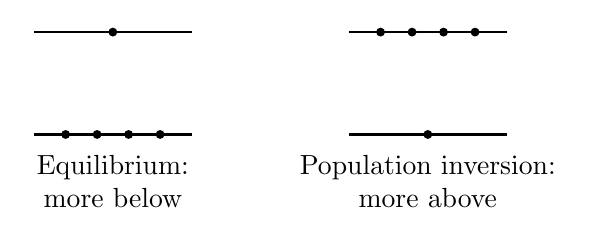
\begin{tikzpicture}
% Thermal equilibrium
\draw[thick] (0,0)--(2.0,0); \draw[thick] (0,1.3)--(2.0,1.3);
\fill (0.4,0) circle (1.6pt); \fill (0.8,0) circle (1.6pt); \fill (1.2,0) circle (1.6pt); \fill (1.6,0) circle (1.6pt);
\fill (1.0,1.3) circle (1.6pt);
\node at (1.0,-0.6) {\shortstack{Equilibrium:\\more below}};
% Inversion
\draw[thick] (4.0,0)--(6.0,0); \draw[thick] (4.0,1.3)--(6.0,1.3);
\fill (5.0,0) circle (1.6pt);
\fill (4.4,1.3) circle (1.6pt); \fill (4.8,1.3) circle (1.6pt); \fill (5.2,1.3) circle (1.6pt); \fill (5.6,1.3) circle (1.6pt);
\node at (5.0,-0.6) {\shortstack{Population inversion:\\more above}};
\end{tikzpicture}
\caption{Each dot is an atom. Equilibrium on the left favors absorption; pumped inversion on the right permits avalanche-like stimulated gain.}
\end{figure}

\begin{mainline}
Read the account backward for spectroscopy, physics' finest mind reader. Unique elemental levels make emission fingerprints. Conversely, continuous light such as stellar thermal radiation crossing cooler gas loses matching photons, making absorption lines. Bright and dark are expenditure and receipt columns of one level account.

Spectroscopy's trophies abound. During the 1868 total eclipse, an unknown yellow solar-chromosphere line signaled helium, named for the Greek Sun and found in terrestrial minerals only over twenty years later. Modern steelworks read sparks from molten steel spectroscopically to report carbon, manganese, and chromium within seconds and guide additions. Forensics compares trace elements in paint and glass; observatories infer composition, temperature, and approach/recession from entire line-set shifts.

Lasers serve barcode scanners, hair-thin-fiber broadband, industrial cutting and welding, and excimer vision surgery. Each ultraviolet photon can break corneal molecular bonds, removing a layer before heat spreads and largely sparing nearby tissue from burns. All exploit denomination, direction, or timing to the fullest.
\end{mainline}

\step{The Model in One Sentence}

\begin{oneline}
Atoms exchange fixed-denomination energy packets set by color. Fluorescence receives larger packets and returns smaller change; lasers first pump population inversion, then use stimulated emission to unify immense numbers of packets' denomination, direction, and timing.
\end{oneline}

\step{The Mathematical Translator}

\begin{mainline}
One denomination formula:
\[
\Delta E=h\nu=\frac{hc}{\lambda}
\]
It gives step height through frequency \(\nu\), wavelength \(\lambda\), Planck's constant \(h\), with \(h\approx 6.63\times10^{-34}\,\mathrm{J\cdot s}\) and \(c\approx 3.0\times10^{8}\,\mathrm{m/s}\). For red \(\lambda\approx 650\,\mathrm{nm}\), \(\nu=c/\lambda\approx 4.6\times10^{14}\,\mathrm{Hz}\) and photon energy \(E\approx 3.1\times10^{-19}\,\mathrm{J}\). Engineering prefers \(1\,\mathrm{eV}\approx 1.6\times10^{-19}\,\mathrm{J}\): red photons are roughly \(1.9\,\mathrm{eV}\), violet at \(\lambda\approx 400\,\mathrm{nm}\) roughly \(3.1\,\mathrm{eV}\).

Check limits. Vanishing frequency, very long radio waves, gives tiny denominations: powerful antennas emit large totals in packets barely disturbing atoms, so radio does not charge your body. Halving wavelength doubles energy, explaining why UV burns skin and charges stickers whereas visible light cannot. Reversal balances: absorbing \(1.9\,\mathrm{eV}\) to rise and descending the same pair returns \(1.9\,\mathrm{eV}\).

How many photons per second from a \(5\,\mathrm{mW}\) red pointer?
\[
N=\frac{P}{E}=\frac{0.005\,\mathrm{J/s}}{3.1\times10^{-19}\,\mathrm{J}}\approx 1.6\times10^{16}\ \text{per second}
\]
As \(P\) vanishes, \(N\) vanishes. At equal \(5\,\mathrm{mW}\), ultraviolet's larger denomination gives fewer photons. A trillion six hundred billion per second sounds formidable, but tiny individual values prevent pointers burning through paper. Yet distant eyes can collect them individually: a few hundred entering a dark-adapted pupil suffice for perception.

% BEGIN TRANSLATOR SAFETY NOTE
\textbf{Translator safety note:} Failure to burn paper does not imply eye safety. Never look into a laser beam or direct it toward an eye, even at the stated low power. See \href{https://www.fda.gov/radiation-emitting-products/alerts-and-notices/illuminating-facts-about-laser-pointers}{FDA's laser-pointer warning}.
% END TRANSLATOR SAFETY NOTE

Fluorescent accounting: absorb a \(400\,\mathrm{nm}\) violet photon, \(3.1\,\mathrm{eV}\); lose \(0.4\,\mathrm{eV}\) internally as heat; emit \(2.7\,\mathrm{eV}\) blue. Emitted photon energy never exceeds incident energy, Stokes' rule. Zero loss returns identical energy, called ordinary scattering rather than fluorescence.
\end{mainline}

\begin{mathbridge}
Why can thermal equilibrium never invert populations? At temperature \(T\), the upper-to-lower ratio is
\[
\frac{N_2}{N_1}=e^{-\Delta E/(kT)}
\]
from Chapter 33's Boltzmann distribution, with \(k\approx 1.38\times10^{-23}\,\mathrm{J/K}\). Check \(T\to 0\): exponent tends negative infinity, everyone downstairs. At \(T\to\infty\), the ratio approaches one, never more upstairs, so heating alone cannot invert. Room-temperature \(kT\approx 1/40\,\mathrm{eV}\), with visible \(\Delta E\approx 2\,\mathrm{eV}\), gives \(e^{-80}\approx 10^{-35}\). Hence room-temperature objects do not emit visible light; filaments need two or three thousand degrees. Selective pumping, current, light, or chemistry, must circumvent equilibrium.

Read, without solving, a three-level rate model. Pumping at \(R\) raises level 1 to short-lived 3, which quickly relaxes nonradiatively into metastable 2. That leaks toward 1 over lifetime \(\tau\):
\[
\frac{dN_2}{dt}=R-\frac{N_2}{\tau}-(\text{stimulated-emission term})
\]
Increase \(R\) and \(N_2\) accumulates into inversion. Stimulated emission grows with intracavity intensity: more light means more invitations and more light, the reinforcing loop and mathematical skeleton of laser oscillation.
\end{mathbridge}

\begin{challenge}
Einstein used spontaneous rate \(A_{21}\), stimulated rate \(B_{21}\rho(\nu)\), and absorption rate \(B_{12}\rho(\nu)\), with \(\rho(\nu)\) radiation energy density near \(\nu\). Equilibrium consistency with Planck forces \(B_{12}=B_{21}\) and \(A_{21}/B_{21}\) proportional to \(\nu^{3}\). Stimulated emission is then no optional assumption but a necessity of balanced atom--radiation accounts. Einstein saw it in 1917, over forty years before lasers.

Now the cavity. A single gain-medium pass of length \(L\) amplifies intensity by \(e^{gL}\), with gain coefficient \(g\). Imperfect mirrors lose some each round trip. Threshold equates single-pass gain and loss. Below it is faint, modestly filtered fluorescence; above it one standing-wave mode avalanches, starving others of inversion. A laser resembles a nonequilibrium phase transition as pump power crosses a critical setting.
\end{challenge}

\begin{mainline}
The same formula explains LED efficiency. Incandescent filaments near three thousand degrees squeeze visible light from thermal emission, wasting most energy as infrared heat. LEDs drop electrons directly across gaps, one photon each, devoting almost all energy to light. Step-height accounting becomes how many packets electricity buys and their denominations.

Finally atomic clocks. The current SI second is 9192631770 periods of radiation corresponding to the cesium-133 ground-state hyperfine transition. Why accuracy of one second over tens of millions of years? Every cesium atom provides the same line, eliminating a locked-away unique artifact; quantum gaps avoid pendulum thermal expansion and quartz aging; and frequency is our most precisely measurable quantity, with counting easier than length or mass metrology.

Satellite navigation famously uses atomic clocks. Signal travel time times light speed gives distance. At roughly three hundred thousand kilometers per second, a one-nanosecond timing error means thirty centimeters. Special and general relativity make satellite clocks net thirty-eight microseconds faster daily. Without Chapters 39 and 41's corrections, error accumulates around ten kilometers per day. Every ride-hailing location relies on joint atomic-clock and relativity duty.
\end{mainline}

\step{The Model's Limits}

\begin{mainline}
Every useful statement needs a boundary.

Lasers are not mathematically single-frequency. Thermal motion and cavity-length fluctuations give finite linewidth. Stabilization makes it narrow, never zero.

Beams are not perfectly parallel. Diffraction from diameter \(D\) imposes divergence around \(\lambda/D\). A one- or two-millimeter pointer aperture makes a coin-sized spot tens of meters away through this limit, not poor construction.

Stimulated cloning copies mode properties, frequency, direction, phase, not arbitrary photon-carried information for superluminal delivery. Chapter 48's no-signaling rule remains.

Two levels plus strong light do not make a laser. Equal-frequency pumping also stimulates descent, at best equalizing populations, not inverting. Real lasers use a third level or directly produce excitation through current or chemistry; semiconductor lasers inject electrons and holes.

Fluorescence is not self-created light. Absorbed light, or current or chemistry, supplies all energy, with output no greater than absorbed input. White shirts appear excessively bright because dark surroundings and invisible UV convert to visible blue, not because energy multiplies.

Light never changes back and forth between wave and particle here. Propagation uses waves, with interference and diffraction; atomic energy exchange uses packets. These are two accounts of one object, like total turnover and itemized receipts for one shop, not changing physical forms.

Classical optics survives. Imaging, reflection, refraction, interference, diffraction, and polarization remain accurate in strong light, the average behavior of immense photon populations. Quantum theory supplies individual exchanges and faint light. A few photons per second still give individual dots that eventually build Chapter 43's fringes. Classical optics is the totals page; quantum theory the transaction ledger.

Two final misuses: lasers do not produce energy. Pumping supplies it, often at under-half electrical-to-optical efficiency, with waste heat requiring substantial cooling. Nor do white LEDs emit white photons; white is the eye's aggregate sensation from mixed photon colors.
\end{mainline}

\begin{figure}[htbp]
\centering
\begin{tikzpicture}[>=Stealth]
\draw[fill=orange!15] (0,0) rectangle (5,1);
\node at (2.5,0.5) {\shortstack{Gain medium\\(population inversion)}};
\draw[line width=2.2pt] (-0.12,-0.45)--(-0.12,1.45);
\node[below] at (-0.12,-0.45) {Full mirror};
\draw[line width=2.2pt] (5.12,-0.45)--(5.12,1.45);
\node[below] at (5.12,-0.45) {Partly transmitting mirror};
\draw[<->,red!70!black] (0.15,0.5)--(4.85,0.5);
\draw[->,red!70!black,line width=1.6pt] (5.12,0.5)--(6.9,0.5) node[right]{Laser output};
\draw[->,blue!70!black,line width=1.2pt] (2.5,2.1)--(2.5,1.08);
\node[above] at (2.5,2.1) {Pump: current or another beam};
\end{tikzpicture}
\caption{Pumping inverts populations; two mirrors form a cavity repeatedly amplifying axial modes. Some light leaves the right mirror as laser output.}
\end{figure}

\step{Explaining the Opening Phenomenon}

\begin{mainline}
Return to the two lights. A flashlight filament radiates thermally through randomly excited atoms, with assorted directions, colors, and timing. Its substantial power spreads thinly across angle and spectrum. A laser pointer's miniature semiconductor receives current-injected electrons and holes, making inversion; parallel cleaved crystal ends form cavity mirrors. Off-axis and nonresonant light leaks away; one surviving mode is repeatedly stimulated and amplified. One mechanism fixes direction, color, and timing, concentrating a few milliwatts into a tiny cone and bandwidth. It is organization, not extra energy. Estimate \(5\,\mathrm{mW}\) laser divergence at a milliradian versus a \(5\,\mathrm{W}\) flashlight spread across much of a hemisphere. A thousandfold power disadvantage meets a millionfold solid-angle advantage, letting laser intensity per direction win by orders, explaining that dazzling twenty-meter spot.

Stickers likewise resolve. Violet denominations lift electrons onto an elevated route with a metastable parking lot before ground. Slow queued descent emits green for minutes after lights go out. Red cannot pay the entry fee, regardless of dazzling intensity: atoms do not accept small change, and more power cannot rescue it.

Settle the guesses: laser purity combines level gaps, cavity modes, and stimulated cloning, not filters or material alone; narrowness combines cavity direction and diffraction; stickers store in metastable parking, not slow reflection; red loses on denomination, not total. How many did you get?
\end{mainline}

\step{Thought Experiments and Challenges}

\begin{thought}[A Few Photons from the Moon]
Since 1969 Apollo astronauts placed lunar corner reflectors. Observatories still send pulses of roughly \(10^{17}\) photons; after a 2.5-second round trip, only a few return on average. Outbound spots already span kilometers, so almost all miss the reflectors.

Yet these survivors measure lunar distance to millimeters and reveal yearly recession near 3.8 centimeters. Why does sending \(10^{17}\) and receiving a few work? Complete recovery is unnecessary; returning photons need only faithfully carry travel time. Each detector click ultimately involves an atom absorbing a photon, light--atom cooperation to the final instant.

Why not make the laser ten thousand times brighter? A few returns already suffice if counting is clean, preserving precise arrival times. Often noise discrimination, not mere weak signal, limits measurement. Purifying laser timing and speeding detector response reduce that noise account.
\end{thought}

\begin{mainline}
This chapter bridges ahead. Nuclear energy steps rise from eV to hundreds of thousands or millions of eV, renaming photons \(\gamma\) rays in Chapter 56. Stimulated photons' indistinguishability advertises Chapter 53's bosons and the modern field picture: photons excite the electromagnetic field, and lasers crowd one mode. This is practical: gravitational-wave instruments repeatedly reflect powerful, exceptionally stable laser light through kilometer arms, measuring length changes thousands of times smaller than a proton and hearing colliding black holes. Light and atoms have only begun their cooperation.
\end{mainline}

\begin{puzzles}
\item Why do shops lack white-light laser pointers? Hint: what two ingredients enforce purity? Could one cavity and inversion simultaneously indulge every color?
\item Bent glow sticks and fireflies emit without prior illumination. Does that violate fluorescence requiring absorbed light? Hint: trace energy. Pumping need not be optical; what other payments fill the elevated reservoir?
\item A brightened white shirt under a banknote lamp stops glowing immediately when it switches off; a sticker lasts ten minutes. Both absorb then emit. Which intermediate step differs? Hint: is there parking, and how wide are its exit lanes?
\item A distant galaxy's lines all shift redward from laboratory hydrogen while retaining hydrogen's relative pattern. Why confidently identify hydrogen, and what might the overall shift report? Hint: pattern identifies elements; whole-pattern displacement is different physics, including Chapter 38's Doppler effect and cosmic expansion.
\end{puzzles}
